\chapter{Estado del Arte}
\section{Alzheimer}
\subsection{¿Qué es?}
La enfermedad de Alzheimer es la principal causa de demencia en personas mayores \cite{donoso2003enfermedad, romano2007enfermedad}. Esta patología presenta una compleja patogenia que, en ocasiones, puede ser hereditaria; se caracteriza por la pérdida progresiva de neuronas y sinapsis, así como por la degeneración neurofibrilar. Clínicamente, el Alzheimer se manifiesta como una demencia de inicio lento e insidioso que usualmente comienza con fallos de memoria y evoluciona hasta comprometer la autonomía total del paciente \cite{merino2015enfermedad}.\\

Los casos de Alzheimer se incrementan con la edad. Raramente se manifiesta antes de los 50 años y tampoco es común en pacientes de 60 años; sin embargo, a medida que se avanza en edad, el número de casos aumenta significativamente, llegando a afectar al 15\%--20\% e incluso al 33\% de las personas mayores de 85 años \cite{donoso2003enfermedad}. En las mujeres la prevalencia de esta enfermedad es mayor debido a diversos factores, entre los que destacan una mayor esperanza de vida respecto a los hombres y la ausencia de estrógenos en la etapa postmenopáusica. Asimismo, se ha observado una correlación adaptativa en pacientes con antecedentes de enfermedades cardiovasculares, hipertensión arterial mal controlada y baja escolaridad. Esto último podría explicarse debido a que una mayor reserva cognitiva y el uso activo de las redes neuronales favorecen los procesos de neurogénesis.\\

La duración de la enfermedad es variable y no está determinada de forma fija; existen casos de pacientes que fallecen antes de los 4 años desde el diagnóstico, mientras que otros sobreviven más de 10 años, situándose el promedio general entre los 7 y 8 años \cite{donoso2003enfermedad}.

\subsection{Síntomas}
La sintomatología no se limita únicamente al deterioro cognitivo, sino que también engloba los denominados síntomas psicológicos y conductuales de la demencia (SPCD), los cuales alteran la percepción, el pensamiento y el estado de ánimo del individuo \cite{romero2018importancia, reyes2010sintomas}. Estos síntomas se dividen en dos categorías: los psicológicos, que abarcan desde delirios y alucinaciones hasta cuadros de depresión y apatía; y los conductuales, relacionados con la agitación, la resistencia a los cuidados, las agresiones verbales y la irritabilidad \cite{romero2018importancia}.\\

El Alzheimer presenta comorbilidades frecuentes, como los trastornos del sueño y el trastorno obsesivo-compulsivo. De hecho, en los criterios diagnósticos establecidos en 1984 para esta enfermedad, el insomnio y los delirios ya figuraban como síntomas asociados de relevancia.\\

Por su parte, la fase prodrómica se define como la etapa sintomática previa a la demencia instaurada. Se caracteriza por manifestaciones que no son lo suficientemente graves como para impedir el desarrollo diario, y se rige principalmente por el criterio central de la alteración de la memoria episódica \cite{valls2010diagnostico}.\\

Durante el curso de la enfermedad se manifiesta el déficit cognitivo como el rasgo clínico más importante, estando presente en la gran mayoría de los pacientes \cite{merino2015enfermedad}. Este déficit afecta de manera prioritaria a la memoria a corto plazo, encargada de registrar situaciones o momentos recientes.\\

A medida que avanza el deterioro funcional, el paciente encuentra dificultades para realizar actividades de la vida cotidiana, tales como recordar conversaciones o asistir a eventos programados (por ejemplo, una cita médica). Con el paso del tiempo, estas limitaciones se agravan de forma progresiva, afectando incluso a la ejecución de las actividades básicas de la vida diaria (ABVD) y al autocuidado.

\subsection{Tratamiento}
En la actualidad no existe una cura para esta enfermedad, por lo que el enfoque terapéutico se compone de tres pilares fundamentales: 
\begin{itemize}
    \item Tratamiento farmacológico.
    \item Estimulación de la actividad cerebral.
    \item Orientación y apoyo familiar.
\end{itemize}

En el marco del tratamiento farmacológico se emplean medicamentos como los inhibidores de la acetilcolinesterasa, los cuales buscan prolongar la disponibilidad de la acetilcolina en la corteza cerebral del paciente. Por otra parte, la administración de estrógenos ha mostrado efectividad preventiva en mujeres sanas. Asimismo, se recurre a psicofármacos como antidepresivos y tranquilizantes para mitigar los trastornos conductuales asociados \cite{merino2015enfermedad}.\\

Se ha demostrado que la actividad cerebral estimula la sinaptogénesis y la neurogénesis, mientras que la inactividad produce el efecto opuesto \cite{castillo2020neuroplasticidad}. Por ello, la estimulación a través de talleres de pintura, baile, juegos de salón o cualquier actividad física y mental resulta de gran importancia para ralentizar el proceso neurodegenerativo.\\

Finalmente, la orientación familiar constituye una parte crítica del tratamiento, dado que el entorno del paciente suele experimentar desconcierto y angustia ante la evolución de la enfermedad, requiriendo preparación y pautas de manejo conductual para afrontar la nueva situación.

\section{Estimulación cognitiva}
La estimulación cognitiva forma parte indispensable del tratamiento no farmacológico para frenar el avance del deterioro \cite{castillo2020neuroplasticidad}. Áreas como la orientación, la atención, las funciones ejecutivas y la concentración son las más beneficiadas en un enfoque terapéutico combinado. A su vez, estas intervenciones mitigan el decaimiento del estado de ánimo, promueven la conciencia de la enfermedad y actúan como factor preventivo frente a la apatía.\\

Combatir el sedentarismo reporta amplios beneficios psicosociales en las personas mayores, favoreciendo el mantenimiento de las funciones cognitivas y la autonomía en las actividades diarias. En este sentido, se ha comprobado la utilidad de los juegos en el desarrollo y preservación de los procesos cognitivos. Específicamente, la estimulación cognitiva asistida por ordenador puede resultar más eficaz que las dinámicas tradicionales, siempre que se mantenga una frecuencia constante \cite{garcia2022eficacia}. De igual modo, el uso de videojuegos interactivos ha demostrado ser beneficioso en la población geriátrica para mejorar parámetros como el equilibrio estático monopodal, consolidándose como una herramienta de soporte significativa en el abordaje de enfermedades neurodegenerativas.\\

Entre las terapias orientadas a la estimulación cognitiva destacan \cite{castillo2020neuroplasticidad}:
\begin{itemize}
    \item \textbf{Terapia de orientación a la realidad:} Consiste en formular preguntas básicas de posicionamiento al paciente para reforzar su estado cognitivo, tales como su nombre, edad, fecha actual, lugar de residencia o ubicación momentánea.
    \item \textbf{Técnica de la reminiscencia:} Se basa en la construcción de un entorno estimulante y confortable que induzca al paciente a evocar y relatar eventos de su pasado.
\end{itemize}

Existen diversos ejercicios validados para la estimulación cognitiva, como los propuestos por Sardinero Peña \cite{pena2010estimulacion}:
\begin{itemize}
    \item \textbf{Líneas superpuestas:} Consiste en relacionar números con letras que se encuentran unidos a través de trazos gráficos. La dificultad radica en que las líneas se cruzan y se superponen entre sí.
        \begin{figure}[H]
        \centering
        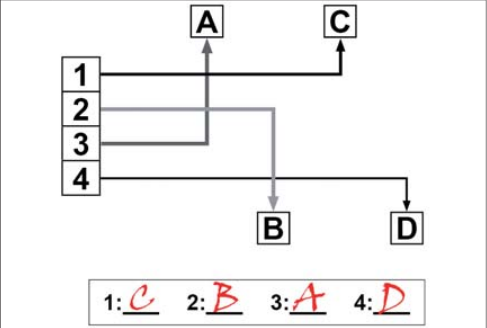
\includegraphics[width=0.7\linewidth]{imagenes/estado_arte/estimulacion/superpuestas.png}
        \caption{Ejercicio de líneas superpuestas.}
        \end{figure}
    \item \textbf{Definiciones:} Requiere la lectura de un enunciado conceptual para posteriormente seleccionar, de entre dos opciones textuales, la palabra exacta que se adecúe a la descripción dada.
    \begin{figure}[H]
        \centering
        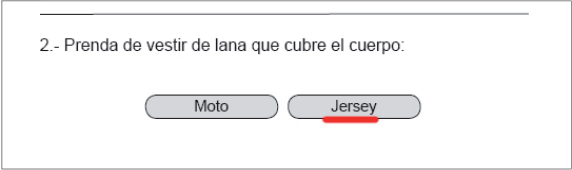
\includegraphics[width=0.7\linewidth]{imagenes/estado_arte/estimulacion/definiciones.png}
        \caption{Juego de definiciones.}
    \end{figure}
    \item \textbf{Completar oración:} El usuario debe elegir una palabra de entre tres opciones posibles para dotar de sentido lógico y sintáctico a la oración presentada en la parte superior.
    \begin{figure}[H]
        \centering
        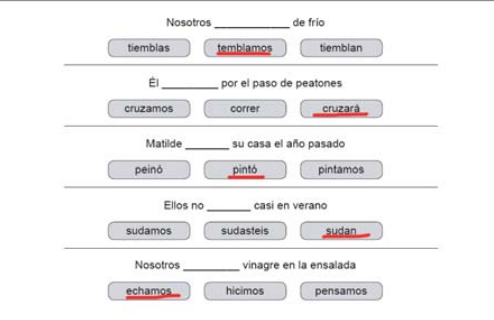
\includegraphics[width=0.7\linewidth]{imagenes/estado_arte/estimulacion/frase.png}
        \caption{Completar oración.}
    \end{figure}
    \item \textbf{El intruso:} Dado un conjunto de imágenes, se debe identificar y seleccionar aquel elemento que no pertenezca a la categoría lógica compartida por los demás.
    \begin{figure}[H]
        \centering
        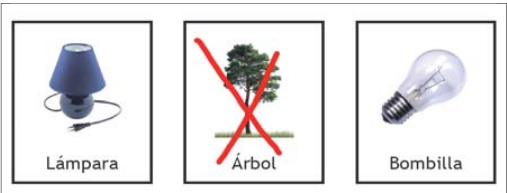
\includegraphics[width=0.7\linewidth]{imagenes/estado_arte/estimulacion/intruso.png}
        \caption{El intruso.}
    \end{figure}
    \item \textbf{Unir números:} Este ejercicio se basa en enlazar de forma secuencial una serie de puntos numéricos mediante líneas en orden creciente.
    \begin{figure}[H]
        \centering
        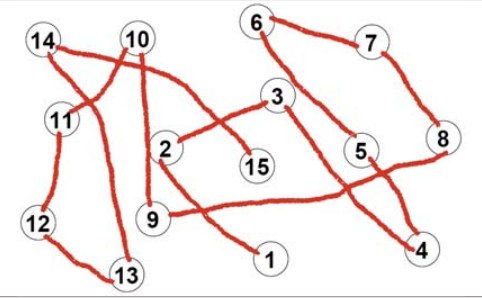
\includegraphics[width=0.7\linewidth]{imagenes/estado_arte/estimulacion/UNIR.png}
        \caption{Unir secuencia de números.}
    \end{figure}
    \item \textbf{Ordenar acciones:} Consiste en organizar cronológicamente un conjunto de ilustraciones que reflejan las fases de una actividad cotidiana, asegurando un resultado coherente.
    \begin{figure}[H]
        \centering
        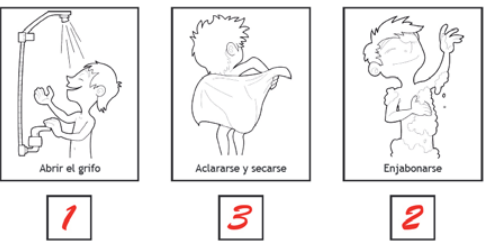
\includegraphics[width=0.7\linewidth]{imagenes/estado_arte/estimulacion/ordenar.png}
        \caption{Ordenar acciones.}
    \end{figure}
\end{itemize}

Adicionalmente, se pueden pautar actividades domiciliarias coordinadas por los cuidadores o familiares, tales como juegos de mesa, dinámicas de cartas, revisión de álbumes fotográficos, ensamblaje de puzles y tareas de jardinería.

\section{Aplicaciones para estimulación cognitiva}

\subsubsection{Constant Therapy}
Constant Therapy es una aplicación desarrollada por la Universidad de Boston que ofrece programas de rehabilitación cognitiva desde el hogar, orientada principalmente a personas que presentan cuadros de demencia o daño cerebral adquirida.\\


Esta plataforma es compatible con smartphones, tablets y chromebooks. Permite realizar un seguimiento sistemático de diversas habilidades cognitivas como la memoria, la percepción visual, la comprensión auditiva, la lectura, la escritura y el cálculo matemático. El programa organiza los ejercicios en diferentes áreas de desarrollo que pueden planificarse de manera personalizada, permitiendo además pausar las sesiones cuando se requiera.\\

La aplicación dispone de una interfaz inicial donde las actividades se encuentran segmentadas por categorías funcionales independientes.
\begin{figure}[H]
    \centering
    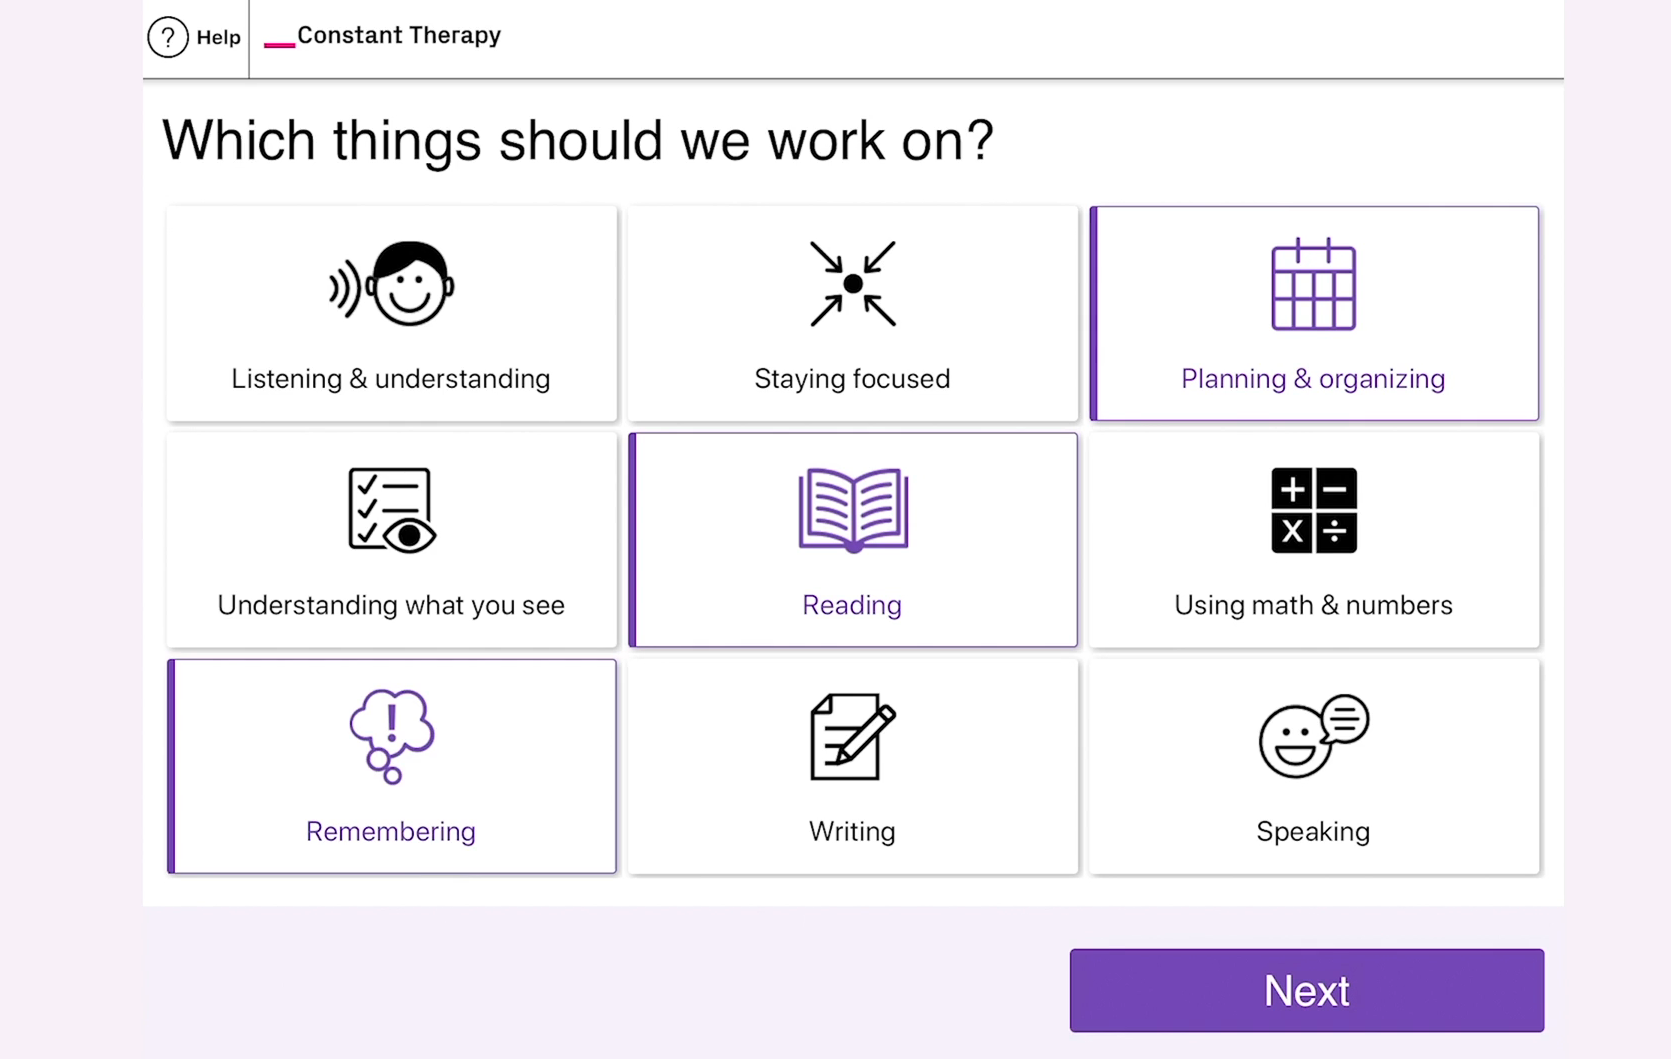
\includegraphics[width=0.7\linewidth]{imagenes/estado_arte/constantTherapy/interfaz.png}
    \caption{Interfaz inicial de la aplicación Constant Therapy.}
    \label{fig:interfaz_constant}
\end{figure}

Entre las tareas que incluye la plataforma se encuentran:
\begin{itemize}
    \setlength{\itemsep}{4pt}
    \setlength{\parskip}{4pt}
    \item Emparejamiento de imágenes ocultas.
    \item Selección de la dirección correcta de estímulos visuales.
    \item Ejercicios de comprensión lectora.
    \item Tareas de respuesta a preguntas basadas en archivos de audio.
    \item Discriminación y localización de símbolos idénticos dentro de conjuntos complejos.
\end{itemize}

El juego de emparejamiento consiste en descubrir imágenes posicionadas boca abajo de forma interactiva. Al hacer clic sobre ellas se revela su contenido, siendo el objetivo memorizar su ubicación espacial para asociarlas de dos en dos.
\begin{figure}[H]
    \centering
    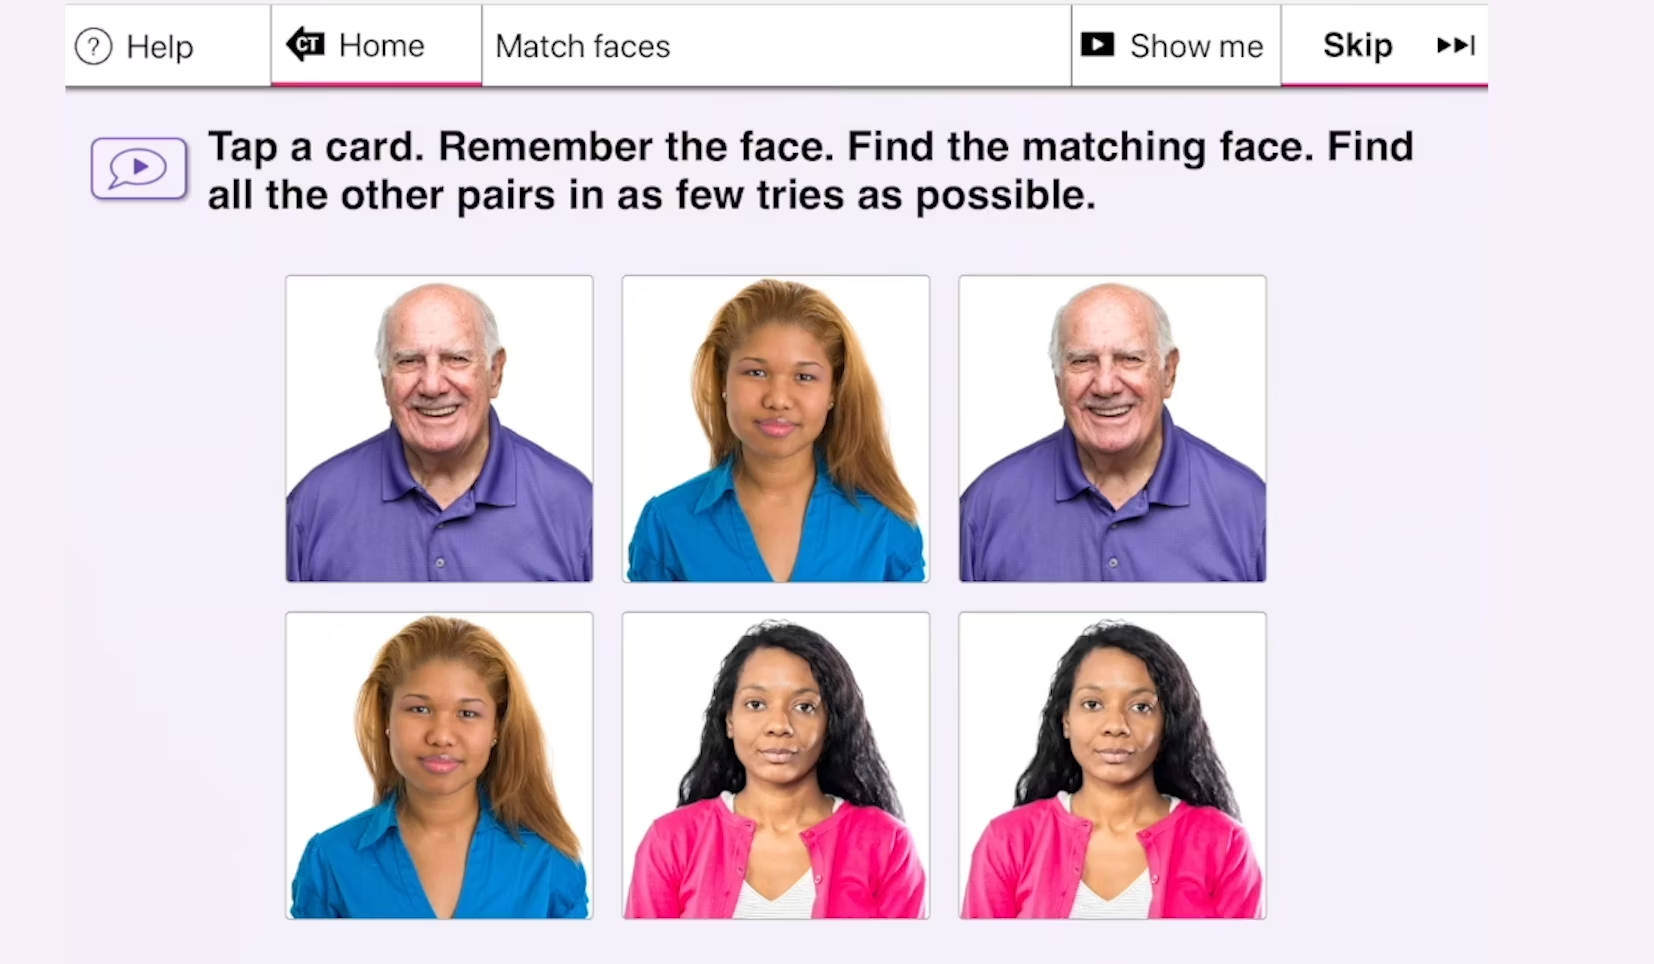
\includegraphics[width=0.7\linewidth]{imagenes/estado_arte/constantTherapy/juego1.png}
    \caption{Juego de emparejamiento en Constant Therapy.}
\end{figure}

Por su parte, las dinámicas de comprensión analizan la capacidad de interpretación del usuario vinculando enunciados textuales con ilustraciones gráficas.
\begin{figure}[H]
    \centering
    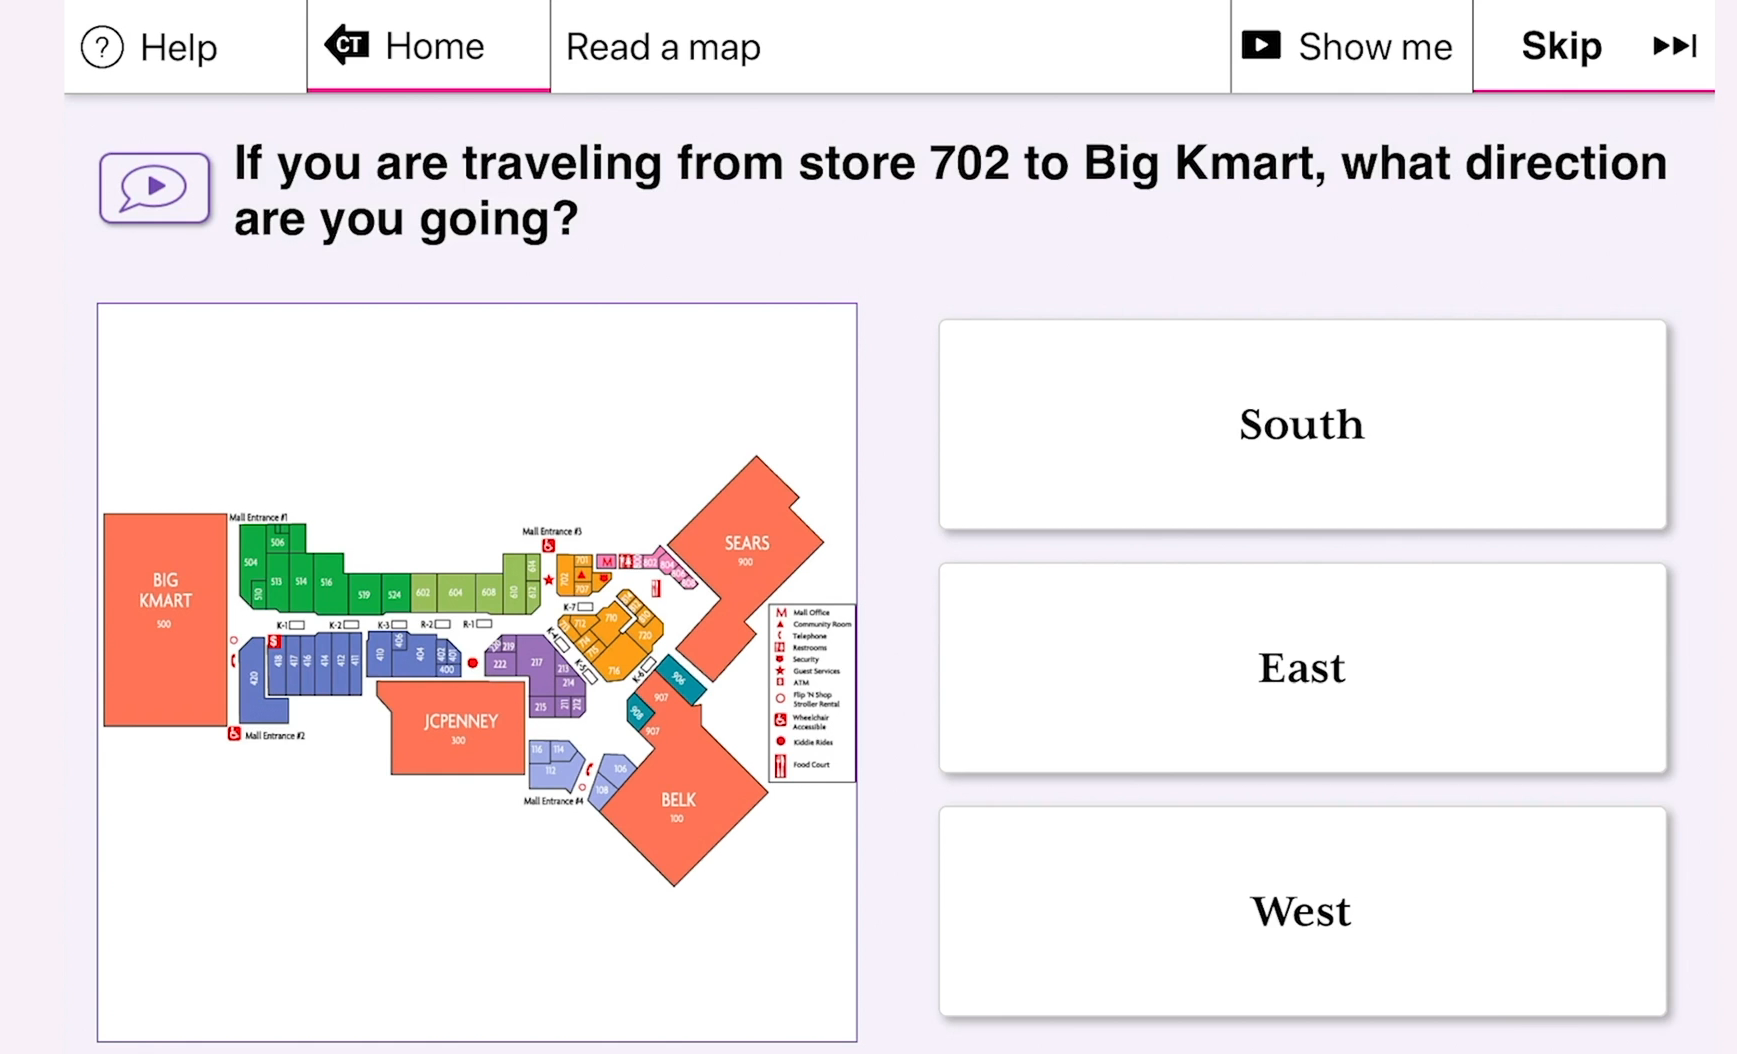
\includegraphics[width=0.7\linewidth]{imagenes/estado_arte/constantTherapy/juego2.png}
    \caption{Ejercicio de asociación imagen-pregunta.}
\end{figure}

Asimismo, se incluyen ejercicios orientados a la selección del término lingüístico que mejor se adecúe a la semántica de una oración propuesta.
\begin{figure}[H]
    \centering
    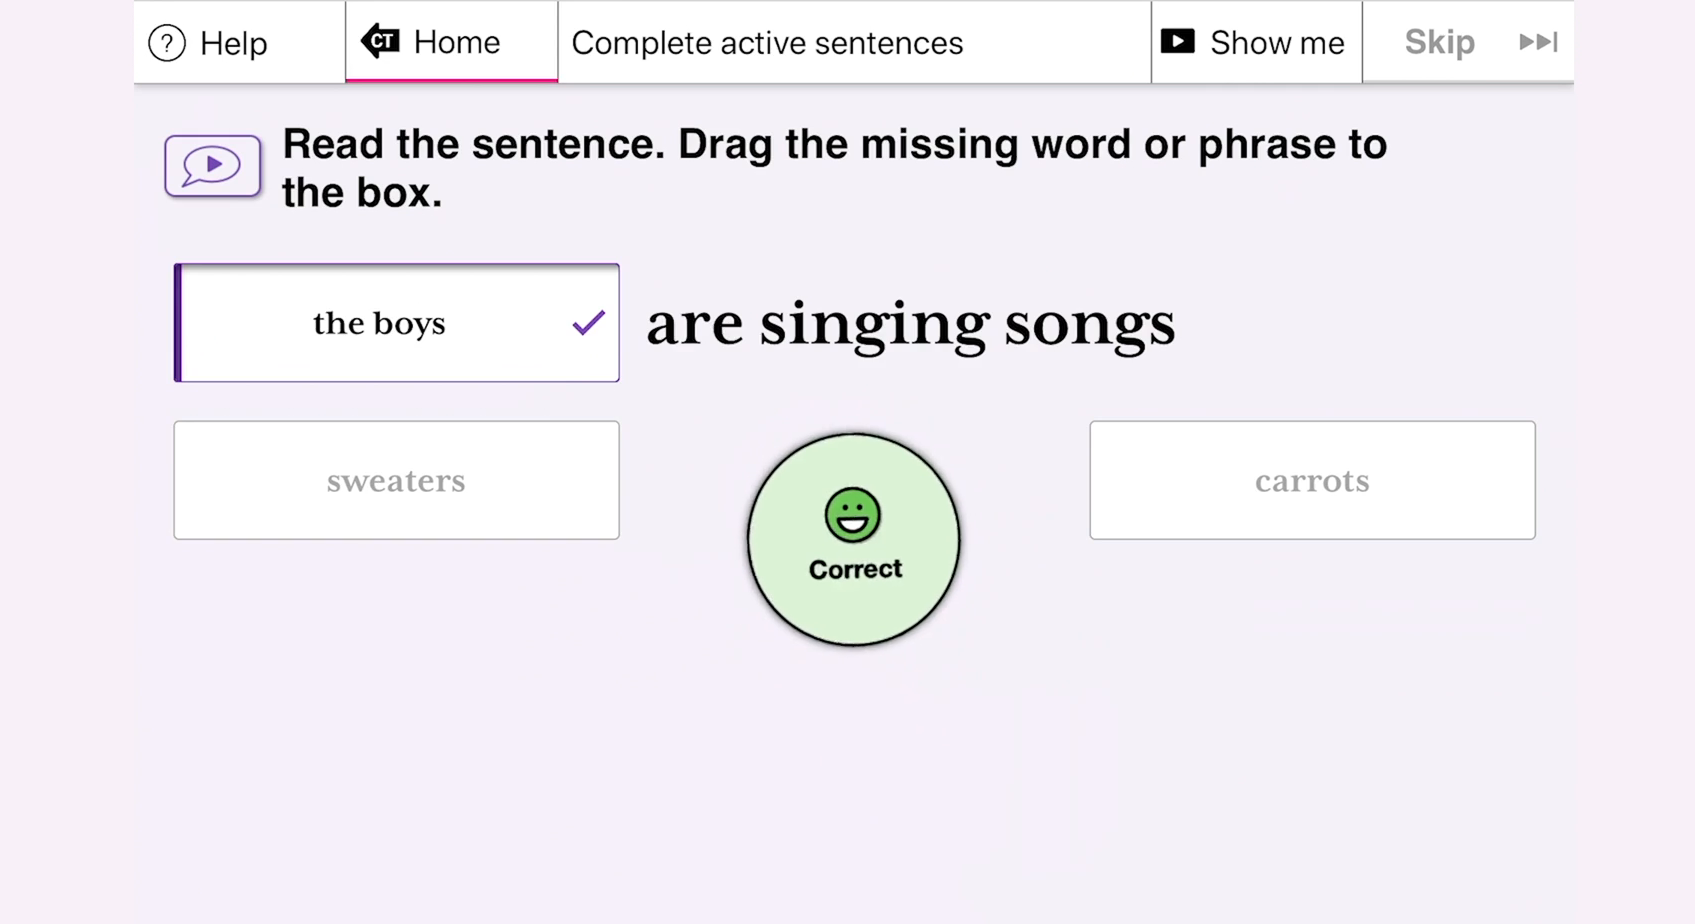
\includegraphics[width=0.7\linewidth]{imagenes/estado_arte/constantTherapy/final.png}
    \caption{Ejercicio de selección de palabras.}
    \label{fig:juego3}
\end{figure}

Otros módulos evalúan de forma específica la comprensión lectora mediante textos breves asociados a imágenes en pantalla.
\begin{figure}[H]
    \centering
    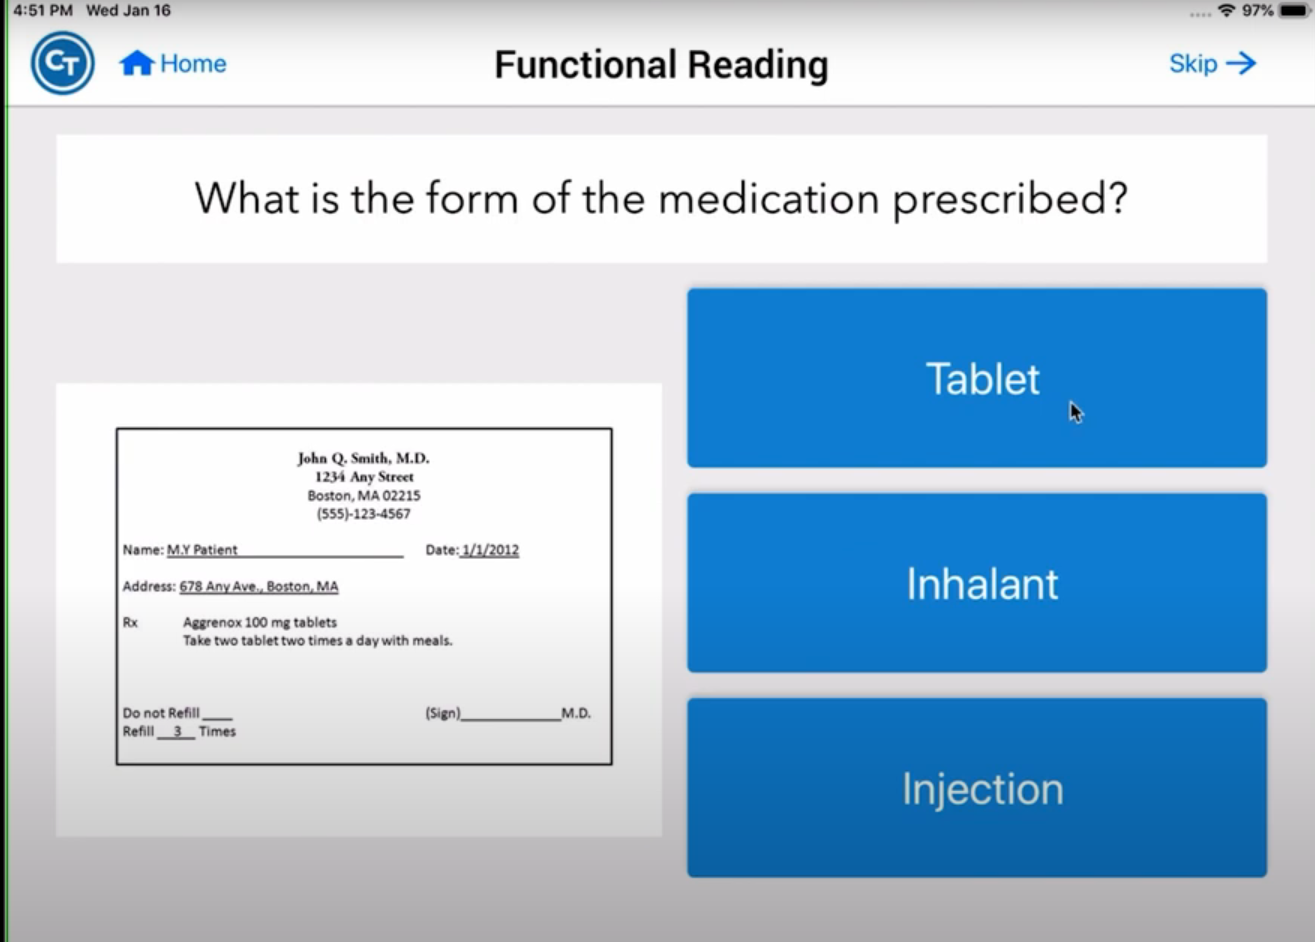
\includegraphics[width=0.7\linewidth]{imagenes/estado_arte/constantTherapy/juego4.png}
    \caption{Evaluación de comprensión lectora.}
    \label{fig:juego4}
\end{figure}
\vspace{-10mm}
\begin{figure}[H]
    \centering
    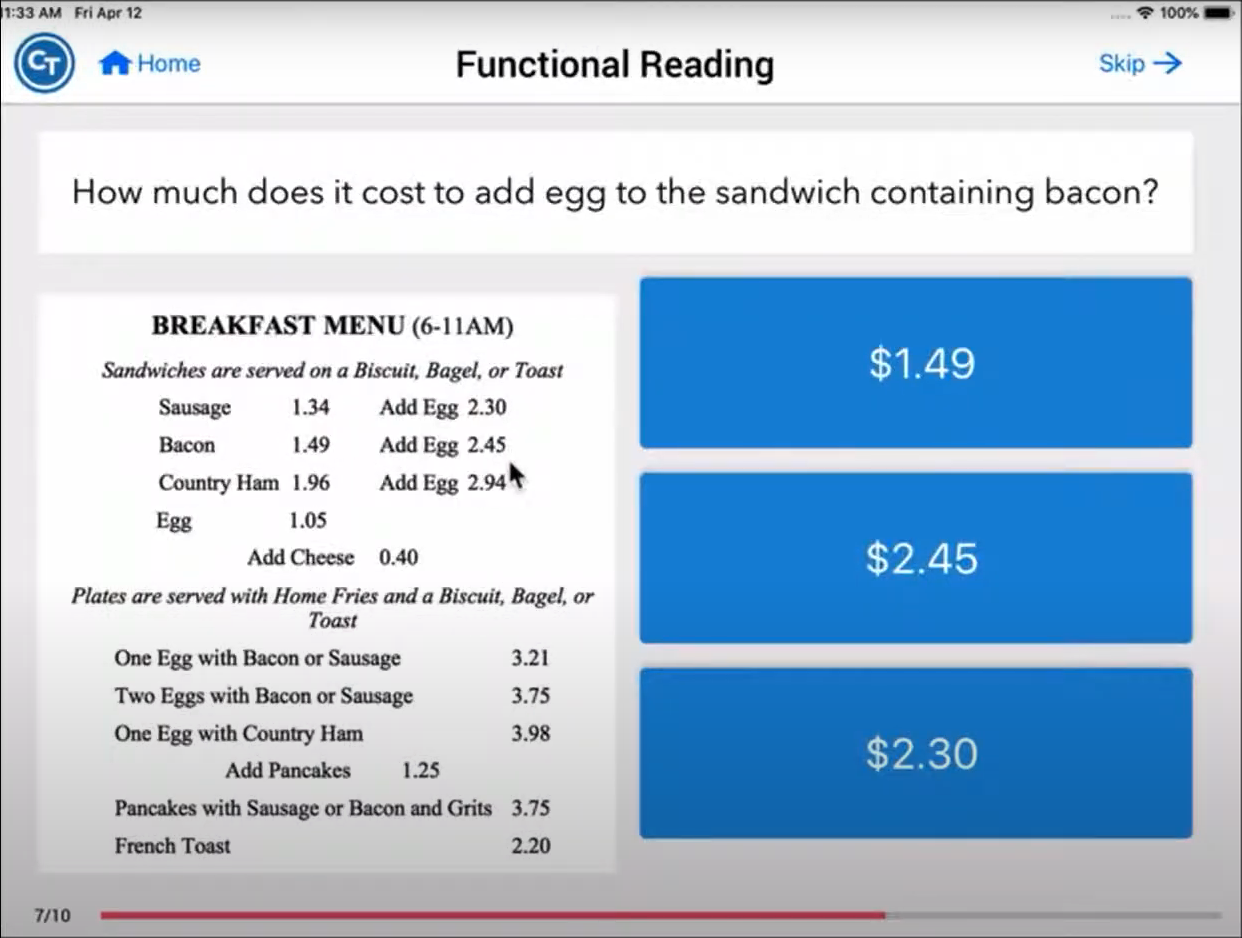
\includegraphics[width=0.7\linewidth]{imagenes/estado_arte/constantTherapy/juego3.png}
    \caption{Variante de ejercicio de comprensión lectora.}
    \label{fig:juego3_var}
\end{figure}

En las tareas de procesamiento auditivo se reproduce un archivo de sonido y el usuario debe relacionar la información escuchada con la pregunta formulada en la pantalla.
\begin{figure}[H]
    \centering
    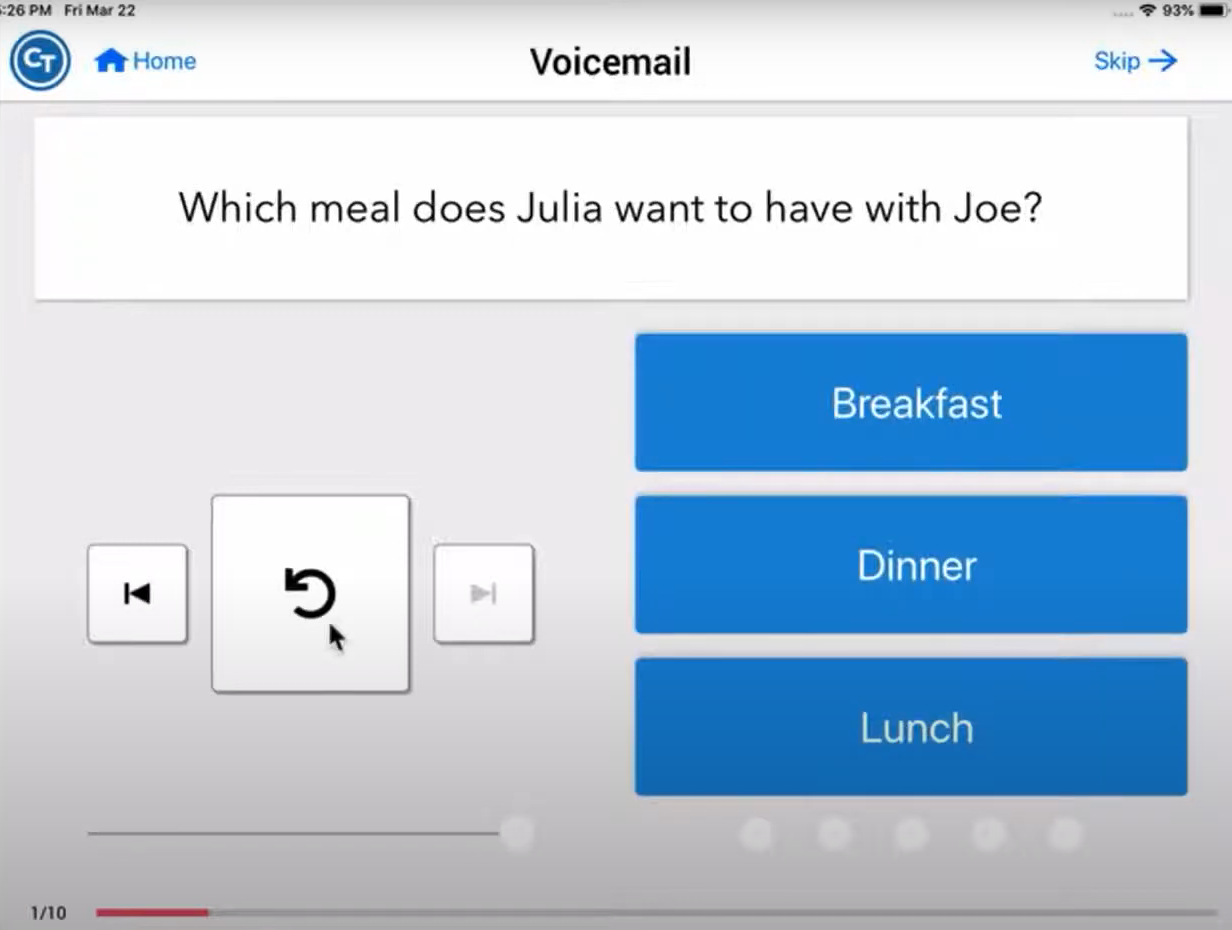
\includegraphics[width=0.7\linewidth]{imagenes/estado_arte/constantTherapy/juego6.png}
    \caption{Ejercicio de comprensión auditiva.}
    \label{fig:juego6}
\end{figure}

Los ejercicios de discriminación visual guardan similitud con el emparejamiento tradicional, pero se centran en la localización ágil de un mismo símbolo o imagen diana oculto entre múltiples distractores concurrentes.
\begin{figure}[H]
    \centering
    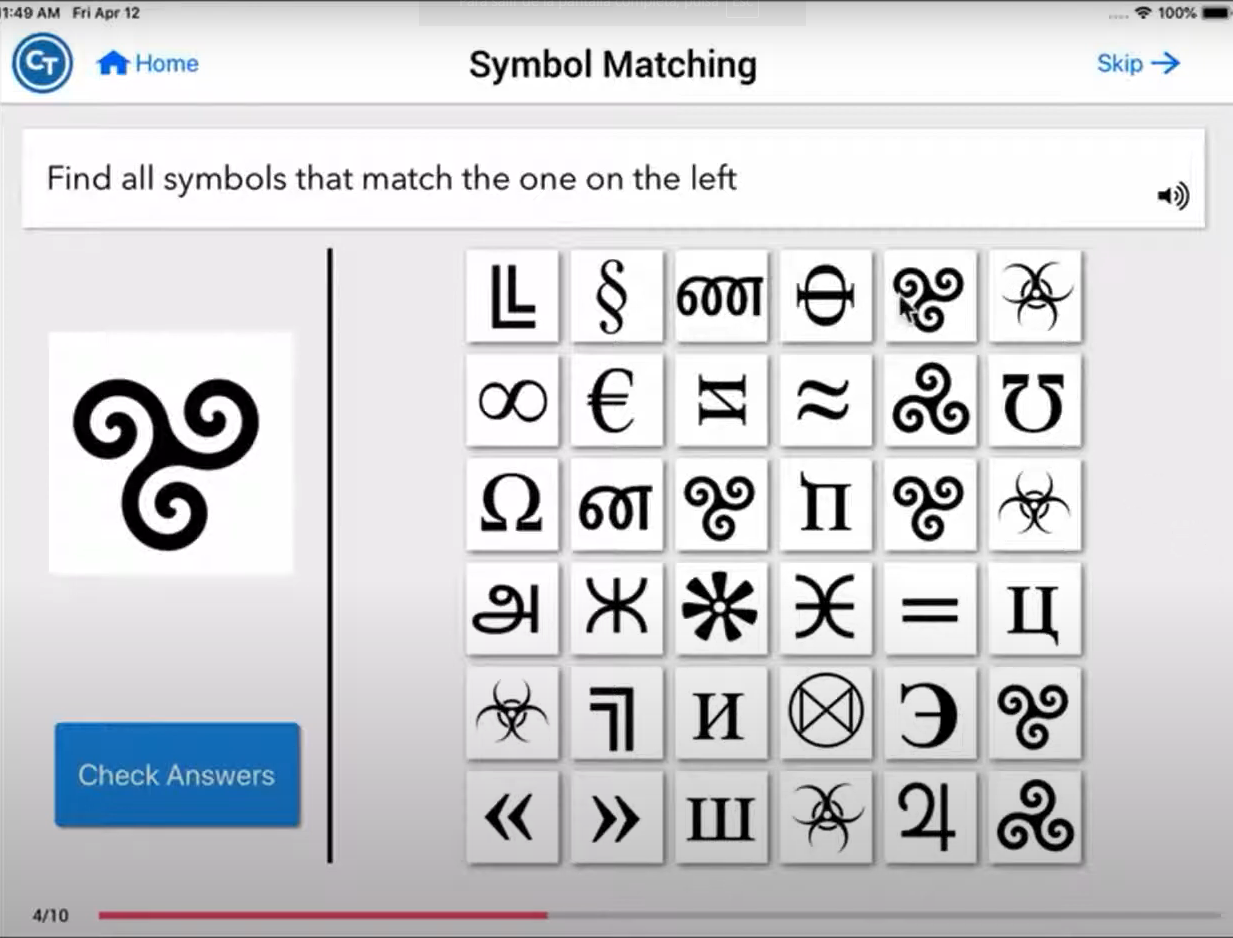
\includegraphics[width=0.7\linewidth]{imagenes/estado_arte/constantTherapy/juego5.png}
    \caption{Ejercicio de búsqueda visual de símbolos.}
    \label{fig:juego5}
\end{figure}

Finalmente, la plataforma incorpora un módulo analítico de estadísticas donde se monitoriza el porcentaje de precisión en los aciertos y el tiempo empleado por el usuario para completar cada sesión de trabajo.
\begin{figure}[H]
    \centering
    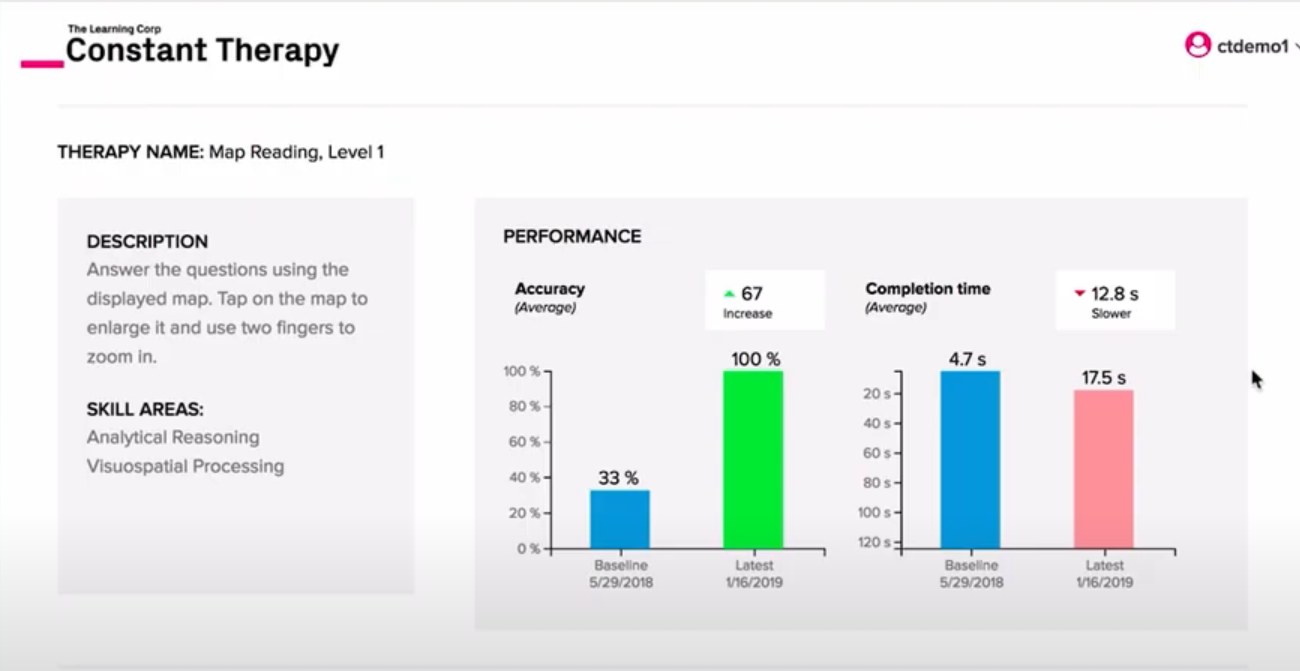
\includegraphics[width=0.7\linewidth]{imagenes/estado_arte/constantTherapy/estadisticas.png}
    \caption{Módulo de visualización de estadísticas del usuario.}
    \label{fig:estadisticas}
\end{figure}

Adicionalmente, al inicio de cada ciclo de entrenamiento se presenta un cuestionario de seguimiento psicométrico que explora de manera subjetiva diferentes ámbitos de la percepción del paciente (por ejemplo, evaluando el nivel de recuerdo respecto a las imágenes visualizadas en la semana anterior).
\begin{figure}[H]
    \centering
    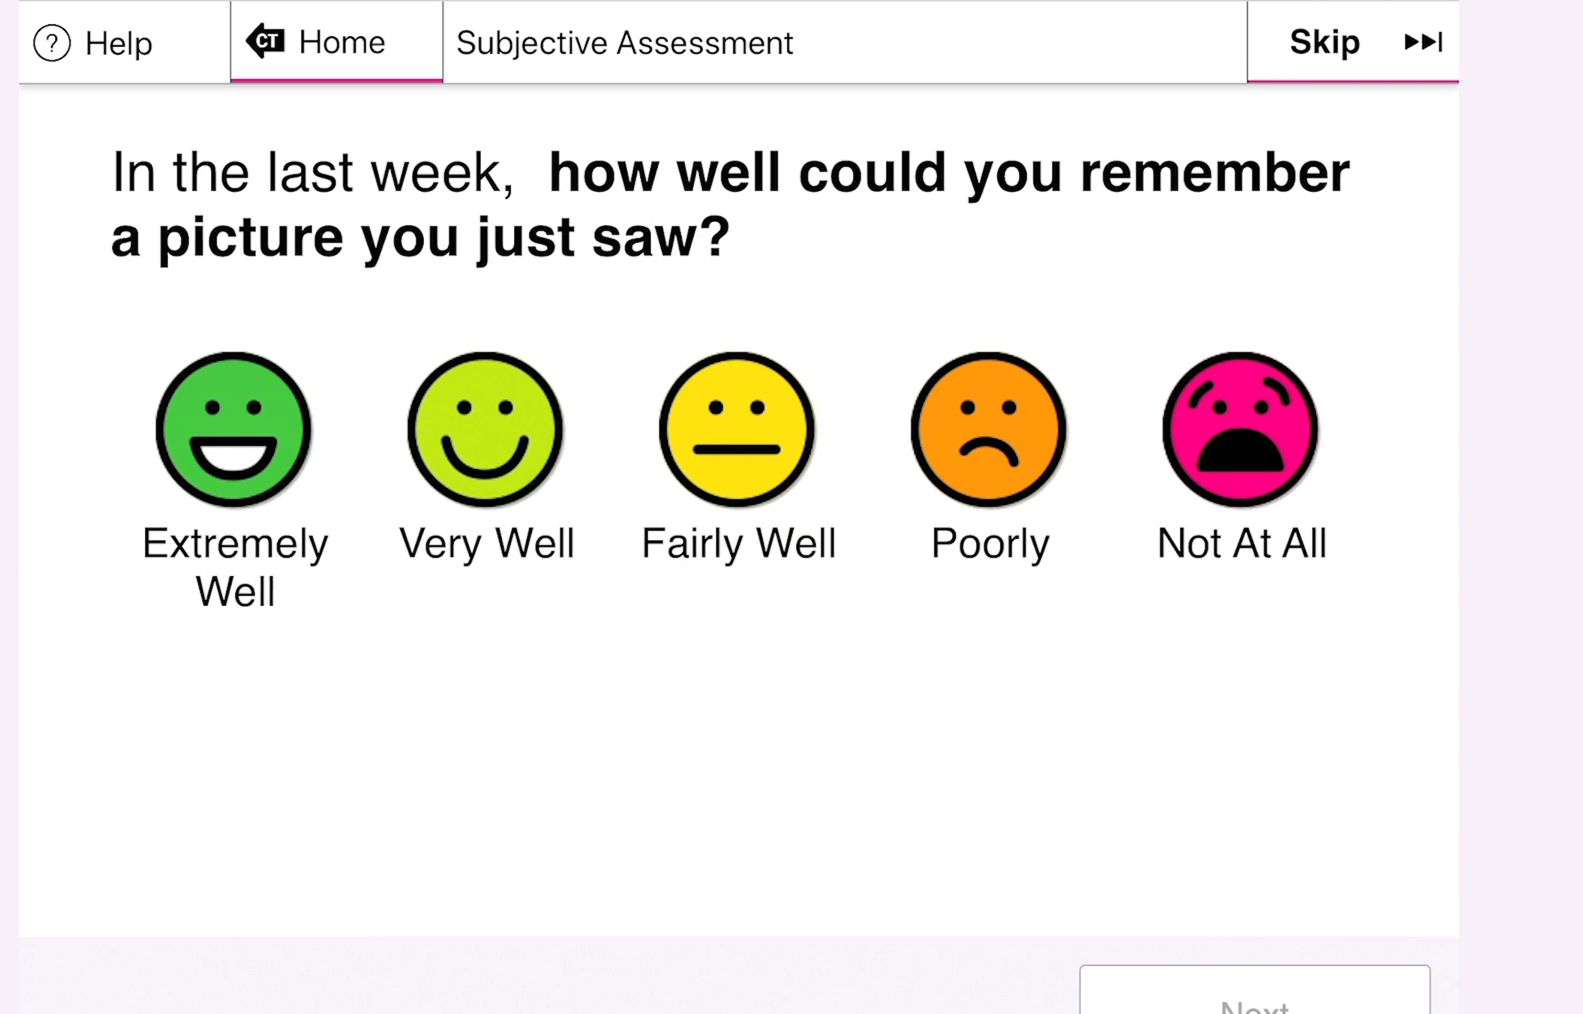
\includegraphics[width=0.7\linewidth]{imagenes/estado_arte/constantTherapy/seguimiento.png}
    \caption{Interfaz de cuestionario de seguimiento semanal.}
    \label{fig:seguimiento}
\end{figure}

\subsection{Limitaciones y áreas de mejora de la plataforma Constant Therapy}
A pesar del respaldo científico y la adopción clínica de \textit{Constant Therapy} en el ámbito de la telerrehabilitación cognitiva y del lenguaje, el análisis de su implementación revela diversas limitaciones estructurales y operativas que condicionan su aplicabilidad en contextos institucionales y particulares:

\begin{itemize}
    \item \textbf{Barreras idiomáticas y de validez ecológica:} La plataforma evidencia un sesgo geocultural al estar optimizada prioritariamente para el inglés norteamericano, lo cual afecta tanto a las consignas auditivas como al algoritmo de reconocimiento de voz. La literatura científica advierte que la traducción de pruebas cognitivas del inglés sin un rigor cultural profundo compromete gravemente la validez y fiabilidad clínica en poblaciones no angloparlantes \cite{dort2020_aphasia}. Asimismo, la falta de estímulos representativos y congruentes con el entorno del paciente (como exigir el uso del sistema monetario estadounidense) reduce drásticamente la validez ecológica de las intervenciones orientadas a las actividades de la vida diaria (AVD) \cite{ellis2022_representation}.
    
    \item \textbf{Rigidez en la transferencia funcional de los estímulos:} El ecosistema de la aplicación no permite la integración de material personalizado (v.g., fotografías de objetos cotidianos o rostros familiares). Investigaciones recientes en neurociencia aplicada a la afasia subrayan que las intervenciones deben ser altamente personalizadas, dado que enfocar la terapia en las necesidades comunicativas únicas de cada individuo es un factor determinante para modular la actividad cerebral y favorecer la plasticidad neuronal \cite{neuroscience_ai_2026}.
    
    \item \textbf{Accesibilidad económica y modelo de monetización:} El modelo de negocio basado en una suscripción recurrente de coste elevado plantea una barrera económica significativa. La literatura destaca que los altos costes directos (\textit{out-of-pocket}) frenan el uso de la salud digital, excluyendo sistemáticamente a poblaciones desfavorecidas \cite{stroke_equity_2021}. A esto se suma el rechazo evidenciado por los usuarios ante modelos poco transparentes (que publicitan descargas gratuitas para posteriormente imponer suscripciones restrictivas de alto valor), lo cual genera ansiedad en pacientes que ya enfrentan la cronicidad \cite{stroke_qualitative_2025}.
    
    \item \textbf{Factores de usabilidad y brecha digital:} La interfaz gráfica demanda el uso casi exclusivo de dispositivos de gran formato (tabletas). Estudios cualitativos realizados con supervivientes de ictus reflejan que las deficiencias visuales y la disminución de la motricidad fina concomitantes a la lesión dificultan enormemente la navegación autónoma por estas interfaces \cite{stroke_qualitative_2025}. La falta de adaptación a la alfabetización tecnológica de los pacientes geriátricos contribuye al aumento de la brecha digital, un fenómeno que empeora progresivamente las desigualdades en salud en la tercera edad \cite{jmir_digitaldivide_2025}.
\end{itemize}

\subsection{Justificación de la propuesta de intervención: El ecosistema ReMind}
Con el propósito de mitigar las carencias identificadas en las plataformas comerciales y garantizar una alternativa viable en el ámbito de la salud digital, se ha diseñado \textit{ReMind}. Esta herramienta ha sido estructurada bajo un paradigma de accesibilidad y continuidad terapéutica, fundamentando su propuesta en dos pilares esenciales:

\begin{enumerate}
    \item \textbf{Resolución de la barrera socioeconómica:} A diferencia de los modelos de suscripción privativos, \textit{ReMind} se constituye como una aplicación de acceso completamente gratuito. Esta gratuidad elimina la segregación por motivos económicos, permitiendo que pacientes con tratamientos de carácter crónico prolonguen su proceso de rehabilitación sin verse condicionados por su capacidad adquisitiva o por la falta de cobertura institucional.
    
    \item \textbf{Optimización del entorno de interacción de hardware:} Frente a la rigidez de los formatos optimizados exclusivamente para dispositivos móviles o tabletas, la arquitectura de \textit{ReMind} ha sido proyectada específicamente para pantallas de ordenador. Esta decisión de diseño amplía sustancialmente el campo visual de los ejercicios, optimizando la ergonomía cognitiva y facilitando el uso a pacientes que presentan de forma concomitante déficits visuales o limitaciones en la motricidad fina. 
\end{enumerate}

La convergencia de estos factores facilita un entrenamiento cognitivo y del lenguaje constante, sistemático y de alta frecuencia, asegurando una mayor adherencia a largo plazo y maximizando los efectos de la neuroplasticidad en la recuperación funcional del usuario.